\section{Supporting Information: Sensitivity in binding free energies due to protein reorganization}
The Supporting Information contains `Simulation Interaction Diagrams' analyzing hydrophobic protein-ligand contacts pertaining to hexylbenzene bound to the protein closed and open state using the default protocol and the pREST protocol.
Tables for each alchemical transformation set have been provided containing the final free energies and inconsistency measurement for each individual transformation.
A link to download the input files for the data set and analysis tools have been provided.
Complete trajectories have been included for the transformations involving benzene to hexylbenzene.


\subsection{Simulation Interactions Diagrams}
Using the `Simulation Interactions Diagram' tool provided with Desmond, we count the number of hydrophobic contacts between the ligand and each of the surrounding protein residues at each frame.
Hydrophobic contacts are categorized into three groups: $\pi$-Cation, $\pi-\pi$, and Other.
The $\pi$-Cation contact is defined as an aromatic and charged group that are within 4.5\AA.
$\pi-\pi$ contacts are when two aromatic groups are stacked face-to-face or face-to-edge.
Hydrophobic contacts that are classified as Other are when hydrophobic side-chains are within 3.6\AA of a ligand's aromatic or aliphatic carbons.

Through this protein-ligand contact analysis, we can see if the ligand forms the same interactions regardless of the initial protein configuration.
In Figure~\ref{fig:contactmap}, we analyze the hydrophobic contacts for hexylbenzene in either the protein closed (purple) or open (green) MD simulations and represent the difference in red.
Here, we represent the number of protein-ligand hydrophobic contacts as a percentage for the length of the MD simulations.
Again, we analyze frames from 0-5ns with the default protocol and 45-55ns with the pREST protocol.

Given hexylbenzene prefers the open conformation, we should expect to see Val111 contact the hexylbenzene at a percent closer to that of the protein open simulation.
Using the default protocol, we show Val111 is in contact with hexylbenzene for 40.4\% of the protein closed simulation and 9.6\% of the protein open simulation, approximately a 30.8\% difference in the interaction percentage.
On the other hand, with the pREST protocol---where Val111 is included into the REST region---this difference dramatically reduces to 0.5\%.
Now, regardless of our initial protein starting conformation, Val111 comes in contact with the ligand 7.9\% and 8.4\% of the protein closed and open simulations, close to what we would have expected judging from our protein open simulation using the default protocol.
Furthermore, we can compute the mean absolute difference (MAD) across all residues to yield 10.5\% for the default protocol and 2.8\% with the pREST protocol.
Overall, the reduction in the difference in protein-ligand contacts indicates the bias from the initial protein configuration is almost entirely eliminated from using pREST.

\setcounter{figure}{0} 
\begin{figure}[!htb]
\begin{subfigure}{\textwidth}
   \centering
   \frame{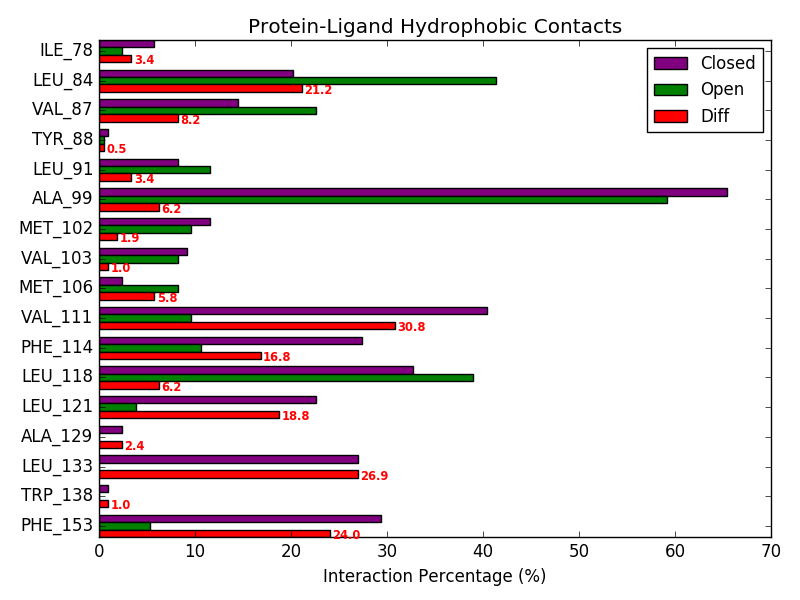
\includegraphics[scale=0.6]{Figures/ContactMap/benzene-hexylbenzene_CM_def.png}}
\end{subfigure}
\centering
\begin{subfigure}{\textwidth}
  \centering
  \frame{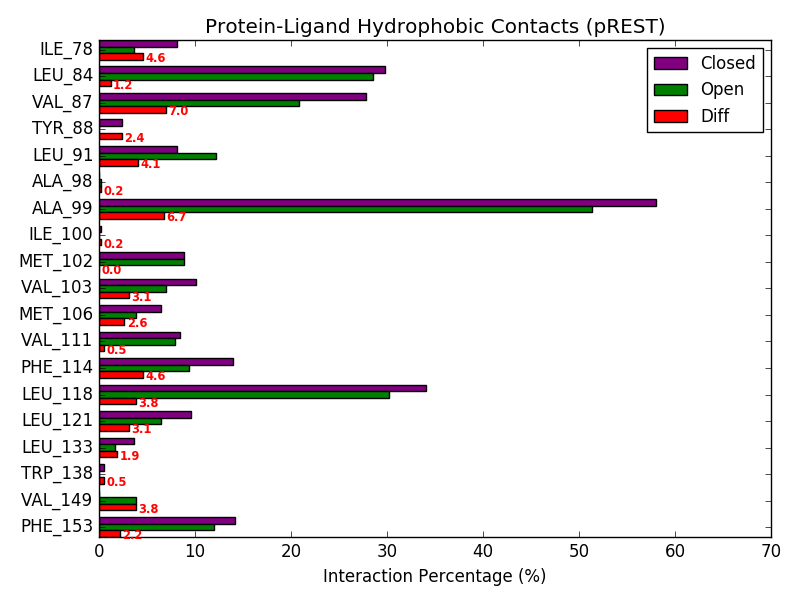
\includegraphics[scale=0.6]{Figures/ContactMap/benzene-hexylbenzene_CM_pREST.png}}
\end{subfigure}
\caption[Protein-ligand hydrophobic contacts]{Bar plot of interaction percentage of protein-ligand hydrophobic contacts over the course of a trajectory. 
From the benzene to hexylbenzene transformation, these plots correspond to the hexylbenzene ($\lambda_{11}$) state from closed (purple) and open (green) simulations using the default versus pREST protocols.
The mean absolute difference (MAD) in interaction percentage is represented in red.
MAD for the default protocol is 10.5\% and 2.8\% for the pREST protocol.
}
\label{fig:contactmap}
\end{figure}

\newpage
\subsection{Tables}

\begin{table}[!htb]
\centering
\caption{Closed-Intermediate Transformations\textsuperscript{\emph{a}}}
\label{tbl:C-I}
\begin{tabular}{|c|c|c|c|c|c|c|}
\hline
\textbf{Ligand 1}   & \textbf{Ligand 2}    & \boldmath$\Delta\Delta G_{C}$ & \boldmath$\sigma_{C}$ & \boldmath$\Delta\Delta G_{O}$ & \boldmath$\sigma_{O}$ & \boldmath$\Delta\Delta G_{\varepsilon}$            \\ \hline
benzene         & butylbenzene   & 0.58    & 0.07  & -0.59  & 0.08  & \cellcolor[HTML]{FFCCC9}1.17 \\ \hline
toluene         & butylbenzene   & -0.28   & 0.06  & -1.27  & 0.09  & \cellcolor[HTML]{9AFF99}0.99 \\ \hline
ethylbenzene    & butylbenzene   & 0.24    & 0.06  & -0.23  & 0.07  & \cellcolor[HTML]{9AFF99}0.47 \\ \hline
propylbenzene & butylbenzene   & 0.99    & 0.06  & 0.63   & 0.04  & \cellcolor[HTML]{9AFF99}0.36 \\ \hline
benzene         & sec-butylbenzene & 2.36    & 0.09  & 2.14   & 0.11  & \cellcolor[HTML]{9AFF99}0.22 \\ \hline
toluene         & sec-butylbenzene & 1.47    & 0.07  & 1.14   & 0.08  & \cellcolor[HTML]{9AFF99}0.33 \\ \hline
ethylbenzene    & sec-butylbenzene & 1.90    & 0.08  & 1.77   & 0.08  & \cellcolor[HTML]{9AFF99}0.13 \\ \hline
propylbenzene & sec-butylbenzene & 2.86    & 0.06  & 2.67   & 0.05  & \cellcolor[HTML]{9AFF99}0.19 \\ \hline
\end{tabular}

\textsuperscript{\emph{a}} Calculated free energies and their uncertainties in `closed-intermediate' alchemical transformations from simulations that were started from the protein closed state(\boldmath$\Delta\Delta G_{C}$) versus the protein open state(\boldmath$\Delta\Delta G_{O}$).
Free energies are in units of kcal/mol. 
The inconsistency(\boldmath$\Delta\Delta G_{\varepsilon}$) is obtained from the difference in the relative free energies between protein closed and open simulations. 
Inconsistency is highlighted red or green if above or below 1 kcal/mol, respectively.
RMSI is 0.6 kcal/mol.
Table is represented in Fig~\ref{fig:C2I_xyplot}.
\end{table}

\begin{table}[!htb]
 \centering
 \caption{Closed-Intermediate Transformations pREST\textsuperscript{\emph{a}}} 
 \label{tbl:C-I_pREST}
 \begin{tabular}{|c|c|c|c|c|c|c|}
 \hline
 \textbf{Ligand 1}       & \textbf{Ligand 2}    & \boldmath$\Delta\Delta G_{C}$ & \boldmath$\sigma_{C}$ & \boldmath$\Delta\Delta G_{O}$ & \boldmath$\sigma_{O}$ & \boldmath$\Delta\Delta G_{\varepsilon}$ \\ \hline
benzene         & butylbenzene   & -0.07   & 0.10     & -0.72     & 0.12     & \cellcolor[HTML]{9AFF99}0.65 \\ \hline
toluene         & butylbenzene   & 0.89    & 0.10     & -0.42     & 0.08     & \cellcolor[HTML]{FFCCC9}1.31 \\ \hline
ethylbenzene    & butylbenzene   & -0.20   & 0.09     & -0.43     & 0.08     & \cellcolor[HTML]{9AFF99}0.23 \\ \hline
propylbenzene & butylbenzene   & 1.02    & 0.06     & 0.49      & 0.06     & \cellcolor[HTML]{9AFF99}0.53 \\ \hline
benzene         & sec-butylbenzene & 0.45    & 0.08     & 1.34      & 0.12     & \cellcolor[HTML]{9AFF99}0.89 \\ \hline
toluene         & sec-butylbenzene & 0.60    & 0.12     & 0.60      & 0.10     & \cellcolor[HTML]{9AFF99}0.00 \\ \hline
ethylbenzene    & sec-butylbenzene & 1.09    & 0.10     & 1.69      & 0.09     & \cellcolor[HTML]{9AFF99}0.60 \\ \hline
propylbenzene & sec-butylbenzene & 1.88    & 0.07     & 3.05      & 0.07     & \cellcolor[HTML]{FFCCC9}1.17 \\ \hline
 \end{tabular}

\textsuperscript{\emph{a}} Calculated free energies and their uncertainties in `closed-intermediate' alchemical transformations from `pREST' simulations that were started from the protein closed state(\boldmath$\Delta\Delta G_{C}$) versus the protein open state(\boldmath$\Delta\Delta G_{O}$).
Free energies were calculated using frames from 0 to 5ns. 
Free energies are in units of kcal/mol.
The inconsistency(\boldmath$\Delta\Delta G_{\varepsilon}$) is obtained from the difference in the relative free energies between protein closed and open simulations. 
Inconsistency is highlighted red or green if above or below 1 kcal/mol, respectively.
RMSI is 0.79 kcal/mol.
Table is represnted in Fig~\ref{fig:C2I_xyplot_pREST}.
 \end{table}

\begin{table}[!htb]
\centering
\caption{Closed-Intermediate Transformations pREST Extended\textsuperscript{\emph{a}},\textsuperscript{\emph{b}}}
\label{tbl:C-I_pRESText}
\begin{tabular}{|c|c|c|c|c|c|c|}
\hline
\textbf{Ligand 1}       & \textbf{Ligand 2}    & \boldmath$\Delta\Delta G_{C}$ & \boldmath$\sigma_{C}$ & \boldmath$\Delta\Delta G_{O}$ & \boldmath$\sigma_{O}$ & \boldmath$\Delta\Delta G_{\varepsilon}$ \\ \hline
benzene          & butylbenzene   & -1.14\textsuperscript{\emph{b}}    & 0.09  & -0.72   & 0.12  & \cellcolor[HTML]{9AFF99}0.42 \\ \hline
toluene          & butylbenzene   & -0.62\textsuperscript{\emph{b}}    & 0.09  & -0.96\textsuperscript{\emph{a}}  & 0.09  & \cellcolor[HTML]{9AFF99}0.34 \\ \hline
ethylbenzene     & butylbenzene   & -0.20     & 0.09  & -0.43   & 0.08  & \cellcolor[HTML]{9AFF99}0.23 \\ \hline
propylbenzene  & butylbenzene   & 0.51\textsuperscript{\emph{b}}     & 0.06  & 0.49    & 0.06  & \cellcolor[HTML]{9AFF99}0.02 \\ \hline
benzene          & sec-butylbenzene & 0.45      & 0.08  & 1.34    & 0.12  & \cellcolor[HTML]{9AFF99}0.89 \\ \hline
toluene          & sec-butylbenzene & 0.60      & 0.12  & 0.60    & 0.10  & \cellcolor[HTML]{9AFF99}0.00 \\ \hline
ethylbenzene     & sec-butylbenzene & 1.09      & 0.10  & 1.69    & 0.09  & \cellcolor[HTML]{9AFF99}0.60 \\ \hline
propylbenzene  & sec-butylbenzene & 1.88      & 0.07  & 1.84\textsuperscript{\emph{b}}   & 0.06  & \cellcolor[HTML]{9AFF99}0.04 \\ \hline
\end{tabular}
 
\textsuperscript{\emph{a}} Calculated free energies and their uncertainties in `closed-intermediate' alchemical transformations from `pREST' simulations that were started from the protein closed state(\boldmath$\Delta\Delta G_{C}$) versus the protein open state(\boldmath$\Delta\Delta G_{O}$).
Free energies were calculated using frames from 15 to 25ns. 
Free energies are in units of kcal/mol.
The inconsistency(\boldmath$\Delta\Delta G_{\varepsilon}$) is obtained from the difference in the relative free energies between protein closed and open simulations. 
Inconsistency is highlighted red or green if above or below 1 kcal/mol, respectively.
RMSI is 0.43 kcal/mol.
Table is represnted in Fig~\ref{fig:C2I_xyplot_pREST}.

\textsuperscript{\emph{b}} Only these alchemical transformations were extended up to 25ns of simulation time in order to lower the inconsistency and error with experiment.
\end{table}

\begin{table}[!htb]
\centering
\caption{Closed-Open Transformations\textsuperscript{\emph{a}}}
\label{tbl:C-O}
\begin{tabular}{|c|c|c|c|c|c|c|}
\hline
\textbf{Ligand 1}       & \textbf{Ligand 2}    & \boldmath$\Delta\Delta G_{C}$ & \boldmath$\sigma_{C}$ & \boldmath$\Delta\Delta G_{O}$ & \boldmath$\sigma_{O}$ & \boldmath$\Delta\Delta G_{\varepsilon}$ \\ \hline
benzene         & pentylbenzene & 2.36       & 0.12  & -1.33  & 0.10  & \cellcolor[HTML]{FFCCC9}3.69 \\ \hline
toluene         & pentylbenzene & 1.77       & 0.09  & 0.34   & 0.10  & \cellcolor[HTML]{FFCCC9}1.43 \\ \hline
ethylbenzene    & pentylbenzene & 2.45       & 0.08  & 0.46   & 0.09  & \cellcolor[HTML]{FFCCC9}1.99 \\ \hline
propylbenzene & pentylbenzene & 3.46       & 0.08  & -0.22  & 0.07  & \cellcolor[HTML]{FFCCC9}3.68 \\ \hline
benzene         & hexylbenzene  & 4.13       & 0.16  & -0.61  & 0.15  & \cellcolor[HTML]{FFCCC9}4.74 \\ \hline
toluene         & hexylbenzene  & 2.90       & 0.13  & -1.63  & 0.08  & \cellcolor[HTML]{FFCCC9}4.53 \\ \hline
ethylbenzene    & hexylbenzene  & 3.63       & 0.11  & -0.76  & 0.09  & \cellcolor[HTML]{FFCCC9}4.39 \\ \hline
propylbenzene & hexylbenzene  & 5.85       & 0.10  & 0.13   & 0.06  & \cellcolor[HTML]{FFCCC9}5.72 \\ \hline
\end{tabular}

\textsuperscript{\emph{a}} Calculated free energies and their uncertainties in `closed-open' alchemical transformations from simulations that were started from the protein closed state(\boldmath$\Delta\Delta G_{C}$) versus the protein open state(\boldmath$\Delta\Delta G_{O}$).
Free energies were calculated using frames from 0 to 5ns.  
Free energies are in units of kcal/mol. 
The inconsistency(\boldmath$\Delta\Delta G_{\varepsilon}$) is obtained from the difference in the relative free energies between protein closed and open simulations. 
Inconsistency is highlighted red or green if above or below 1 kcal/mol, respectively.
RMSI is 4.0 kcal/mol.
Table is represented in Fig~\ref{fig:C2O_xyplot}.
\end{table}

\begin{table}[!htb]
\centering
\caption{Closed-Open Transformations pREST\textsuperscript{\emph{a}}}
\label{tbl:C-O_pREST}
\begin{tabular}{|c|c|c|c|c|c|c|}
\hline
\textbf{Ligand 1}       & \textbf{Ligand 2}    & \boldmath$\Delta\Delta G_{C}$ & \boldmath$\sigma_{C}$ & \boldmath$\Delta\Delta G_{O}$ & \boldmath$\sigma_{O}$ & \boldmath$\Delta\Delta G_{\varepsilon}$\\ \hline
benzene         & pentylbenzene & 1.49       & 0.13     & 0.07   & 0.10     & \cellcolor[HTML]{FFCCC9}1.42 \\ \hline
toluene         & pentylbenzene & 1.41       & 0.12     & 0.79   & 0.13     & \cellcolor[HTML]{9AFF99}0.62 \\ \hline
ethylbenzene    & pentylbenzene & 2.90       & 0.10     & 1.23   & 0.09     & \cellcolor[HTML]{FFCCC9}1.67 \\ \hline
propylbenzene & pentylbenzene & 4.25       & 0.09     & 1.01   & 0.07     & \cellcolor[HTML]{FFCCC9}3.24 \\ \hline
benzene         & hexylbenzene  & 2.75       & 0.14     & 1.25   & 0.11     & \cellcolor[HTML]{FFCCC9}1.50 \\ \hline
toluene         & hexylbenzene  & 3.22       & 0.11     & -1.15  & 0.11     & \cellcolor[HTML]{FFCCC9}4.37 \\ \hline
ethylbenzene    & hexylbenzene  & 3.34       & 0.12     & -0.22  & 0.11     & \cellcolor[HTML]{FFCCC9}3.56 \\ \hline
propylbenzene & hexylbenzene  & 4.93       & 0.12     & 1.21   & 0.11     & \cellcolor[HTML]{FFCCC9}3.72 \\ \hline
\end{tabular}

\textsuperscript{\emph{a}} Calculated free energies and their uncertainties in `closed-open' alchemical transformations from `pREST' simulations that were started from the protein closed state(\boldmath$\Delta\Delta G_{C}$) versus the protein open state(\boldmath$\Delta\Delta G_{O}$).
Free energies are in units of kcal/mol. 
The inconsistency(\boldmath$\Delta\Delta G_{\varepsilon}$) is obtained from the difference in the relative free energies between protein closed and open simulations. 
The inconsistency is highlighted red or green if above or below 1 kcal/mol, respectively.
RMSI is 2.82 kcal/mol. 
\end{table}

\begin{table}[!htb]
\centering
\caption{Closed-Open Transformations pREST Extended\textsuperscript{\emph{a}}}
\label{tbl:C-O_pREST-40-55ns}
\begin{tabular}{|c|c|c|c|c|c|c|}
\hline
\textbf{Ligand 1}       & \textbf{Ligand 2}    & \boldmath$\Delta\Delta G_{C}$ & \boldmath$\sigma_{C}$ & \boldmath$\Delta\Delta G_{O}$ & \boldmath$\sigma_{O}$ & \boldmath$\Delta\Delta G_{\varepsilon}$ \\ \hline
benzene         & pentylbenzene & 1.37       & 0.08     & 1.41    & 0.08      & \cellcolor[HTML]{9AFF99}0.04 \\ \hline
toluene         & pentylbenzene & 1.08       & 0.08     & 0.81    & 0.07      & \cellcolor[HTML]{9AFF99}0.27 \\ \hline
ethylbenzene    & pentylbenzene & 1.71       & 0.08     & 1.50    & 0.07      & \cellcolor[HTML]{9AFF99}0.21 \\ \hline
propylbenzene & pentylbenzene & 3.20       & 0.06     & 2.34    & 0.05      & \cellcolor[HTML]{9AFF99}0.86 \\ \hline
benzene         & hexylbenzene  & 2.15       & 0.09     & 1.14    & 0.08      & \cellcolor[HTML]{FFCCC9}1.01 \\ \hline
toluene         & hexylbenzene  & 0.32       & 0.10     & 1.10    & 0.07      & \cellcolor[HTML]{9AFF99}0.78 \\ \hline
ethylbenzene    & hexylbenzene  & 1.96       & 0.08     & 2.17    & 0.07      & \cellcolor[HTML]{9AFF99}0.21 \\ \hline
propylbenzene & hexylbenzene  & 3.38       & 0.07     & 3.12    & 0.06      & \cellcolor[HTML]{9AFF99}0.26 \\ \hline
\end{tabular}

\textsuperscript{\emph{a}} Calculated free energies and their uncertainties in `closed-open' alchemical transformations from extended `pREST' simulations that were started from the protein closed state(\boldmath$\Delta\Delta G_{C}$) versus the protein open state(\boldmath$\Delta\Delta G_{O}$). 
Free energies are in units of kcal/mol.
Free energies were calculated using frames from 40 to 55ns. 
The inconsistency(\boldmath$\Delta\Delta G_{\varepsilon}$) is obtained from the difference in the relative free energies between protein closed and open simulations. 
Inconsistency is highlighted red or green if above or below 1 kcal/mol, respectively.
RMSI is 0.57 kcal/mol.
Table is represented in Fig~\ref{fig:C2O_xyplot_pREST}.
\end{table}

\begin{table}[!htb]
\centering
\caption{Experimental Ligand Transformations\textsuperscript{\emph{a}}}
\label{tbl:exp_set}
\begin{tabular}{|c|c|c|c|c|c|c|c|}
\hline
\textbf{Ligand 1} & \textbf{Ligand 2}  & \boldmath$\Delta G_{exp}$  & \boldmath$\sigma_{exp}$ & \boldmath$\Delta\Delta G_{C}$ & \boldmath$\sigma_{C}$ & \boldmath$\Delta\Delta G_{O}$ & \boldmath$\sigma_{O}$ \\ \hline
benzene         & toluene         & -0.33        & 0.16            & 0.71       & 0.04          & 0.59       & 0.05          \\ \hline
benzene         & ethylbenzene    & -0.19        & 0.17            & 0.15       & 0.05          & -0.09      & 0.06          \\ \hline
benzene         & propylbenzene & -1.36        & 0.16            & -0.82      & 0.06          & -0.69      & 0.08          \\ \hline
benzene         & butylbenzene  & -1.51        & 0.16            & 0.58       & 0.07          & -0.59      & 0.08          \\ \hline
toluene         & ethylbenzene    & -0.24        & 0.08            & -0.59      & 0.04          & -0.40      & 0.05          \\ \hline
toluene         & propylbenzene & -1.03        & 0.04            & -2.21      & 0.05          & -0.89      & 0.05          \\ \hline
toluene         & butylbenzene  & -1.18        & 0.04            & -0.28      & 0.06          & -1.27       & 0.09         \\ \hline
ethylbenzene    & propylbenzene & -0.79        & 0.07            & -0.86      & 0.05          & -0.80       & 0.03         \\ \hline
ethylbenzene    & butylbenzene  & -0.94        & 0.07            & 0.24       & 0.06          & -0.23      & 0.07          \\ \hline
propylbenzene & butylbenzene  & -0.15        & 0.03            & 0.99       & 0.06          & 0.63       & 0.04          \\ \hline
\end{tabular}

\textsuperscript{\emph{a}} Experimental and calculated free energies with their uncertainties in alchemical transformations involving ligands with available experimental affinities.
Calculated free energies are from simulations that were started from the protein closed state(\boldmath$\Delta\Delta G_{C}$) versus the protein open state(\boldmath$\Delta\Delta G_{O}$). 
Free energies are in units of kcal/mol.
Here, we compare \boldmath$\Delta\Delta G_{C}$ and \boldmath$\Delta\Delta G_{O}$ against \boldmath$\Delta G_{exp}$ to compute the error with experiment.
RMSE is 1.0 kcal/mol and 0.58 kcal/mol for closed and open simulations, respectively.
RMSI is 0.68 kcal/mol.
Table is represented in Fig~\ref{fig:exp_xyplot}.
\end{table}

\begin{table}[!htb]
\centering
\caption{Experimental Ligand Transformations pREST\textsuperscript{\emph{a}}}
\label{tbl:exp_pREST_set}
\begin{tabular}{|c|c|c|c|c|c|c|c|}
\hline
\textbf{Ligand 1} & \textbf{Ligand 2} & \boldmath$\Delta G_{exp}$  & \boldmath$\sigma_{exp}$ & \boldmath$\Delta\Delta G_{C}$ & \boldmath$\sigma_{C}$ & \boldmath$\Delta\Delta G_{O}$ & \boldmath$\sigma_{O}$ \\ \hline
benzene         & toluene         & -0.33 & 0.16  & 0.10  & 0.08  & 0.31  & 0.06          \\ \hline
benzene         & ethylbenzene    &-0.19  & 0.17  & -0.20 & 0.08  & -0.62 & 0.08          \\ \hline
benzene         & propylbenzene & -1.36 & 0.16  & -1.57 & 0.09  & -1.26 & 0.09         \\ \hline
benzene         & butylbenzene  & -1.51 & 0.16  & -1.14 & 0.11  & -0.72 & 0.12         \\ \hline
toluene         & ethylbenzene    & -0.24 & 0.08  & -0.84 & 0.07  & -0.83 & 0.07          \\ \hline
toluene         & propylbenzene & -1.03 & 0.04  & -1.91 & 0.09  & -1.44 & 0.08          \\ \hline
toluene         & butylbenzene  & -1.18 & 0.04  & -0.62 & 0.09  & -0.96 & 0.09          \\ \hline
ethylbenzene    & propylbenzene & -0.79 & 0.07  & -1.08 & 0.07  & -0.80 & 0.06         \\ \hline
ethylbenzene    & butylbenzene  & -0.94 & 0.07  & -0.20 & 0.09  & -0.43 & 0.08         \\ \hline
propylbenzene & butylbenzene  & -0.15 & 0.03  & 0.51  & 0.06  & 0.49  & 0.06       \\ \hline
\end{tabular}

\textsuperscript{\emph{a}} Experimental and calculated free energies with their uncertainties in alchemical transformations involving ligands with available experimental affinities.
Calculated free energies are from `pREST' simulations that were started from the protein closed state(\boldmath$\Delta\Delta G_{C}$) versus the protein open state(\boldmath$\Delta\Delta G_{O}$). 
Free energies are in units of kcal/mol.
Here, we compare \boldmath$\Delta\Delta G_{C}$ and \boldmath$\Delta\Delta G_{O}$ against \boldmath$\Delta G_{exp}$ to compute the error with experiment.
RMSE is 0.54 kcal/mol and 0.50 kcal/mol for closed and open simulations, respectively.
RMSI is 0.31 kcal/mol.
Table is represented in Fig~\ref{fig:exp_xyplot_pREST}.
\end{table}

\clearpage
\subsection*{Data Sets and Analysis Tool Download}
All related data sets and analysis tools are available online and described below.
The files can be downloaded at http://n2t.net/ark:/b7280/d1js3b (doi:10.7280/D1JS3B). 
\begin{description}
\item [Prepared protein-ligand crystal structures:]\texttt{xtal\_prepped.tar.gz}\\
Contains the reference protein-ligand crystal structures that have been aligned and prepared through the `Protein Preparation Wizard' tool as \texttt{.mae} files.
\item [RMSD analysis:]\texttt{scripts.tar.gz}\\
Contains the scripts \texttt{RMSD-analysis.tcl} and \texttt{plot-RMSD.py} used for RMSD analysis. A \texttt{README.txt} file has been provided which details how to generate the RMSD/time and Colormap plots found in the paper. 
\item [FEP data:]\texttt{C-I\_default.tar.gz}, \texttt{C-I\_pPREST.tar.gz}, \texttt{C-O\_default.tar.gz}, \\ \texttt{C-O\_pREST.tar.gz}, \texttt{EXP\_default.tar.gz,} and \texttt{EXP\_pREST.tar.gz}\\
Contains archived data from the FEP calculations for each alchemical transformation set, where within each archived set are directories for individual FEP calculations. These contain input \texttt{.mae} files containing the protein/ligand structures, the simulation configuration \texttt{.msj} files, energy files, and a \texttt{README.txt} that summarizes information about each FEP calculation. Complete trajectories are included.
\end{description}

